\section{Implementacja bazy danych w środowisku MongoDB}
Celem implementacji było stworzenie zestawu replik skłądającego się z 3 procesów \textit{mongod} działających na niezależnych instancjach. 

\subsection{Infrastruktura}
\subsubsection{Instancje}
Baza danych oparta została o chmurę \textit{Azure} w modelu IaaS i \textit{infrastruktura jako usługa}.\\
Utworzone zostały 3 maszyny wirtualne z wykorzystanim obrazów dostarczanych przez \textit{Bitnami}. Systemem operacyjnym działającym na maszynach wirtualnych jest Ubuntu 14.04, natomiast wersja MongoDB to 3.4.0-0. \\

\subsubsection{Sieć wewnętrzna}
Maszyny wirtualne zostały połączone przez prywatną sieć wirtualną, zilustrowaną poniżej. 

\begin{figure}[H]
	\centering
	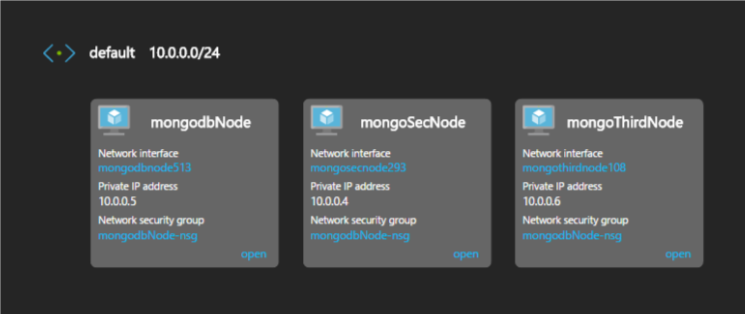
\includegraphics[scale=0.5]{privateNetwork}
	\caption{Sieć wirtualna}
	\label{fig:test}
\end{figure}

\subsubsection{Sieć publiczna}
Aby umożliwić połączenie z zestawem replik od dowolnego klienta, bez wymogu jego wdrożenia w chmurze \textit{Azure}, każdej z instancji maszyn wirtualnych został przydzielony publiczny adres IP, oraz nazwa DNS umożliwiająca dostęp do maszyn.

\subsection{Konfiguracja MongoDB}
Korzystając z \textit{mongo shell} utworzony został zestawe replik następującymi komendami: \\ \\
rs.initiate(); \\
rs.add("10.0.0.4:27017"); \\ 
rs.add("10.0.0.6:27017"); \\ \\

Korzystając z pliku konfiguracyjnego uaktywiono prosty interfejs REST, pozwalający na łatwą diagnozę zestawu replik.

\begin{figure}[H]
	\centering
	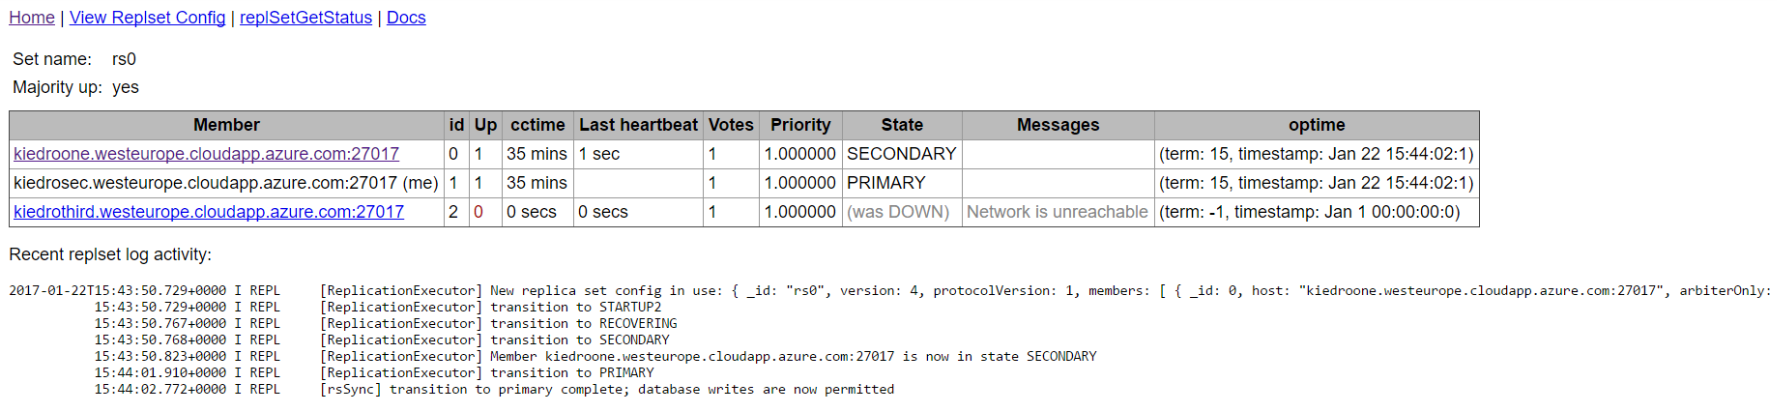
\includegraphics[scale=0.5]{rest_interface}
	\caption{Interfejs REST}
\end{figure}